\documentclass[11pt,a4paper]{article}

\usepackage[T1]{fontenc}
\usepackage{lmodern}
\usepackage[a4paper,margin=2.3cm]{geometry}
\usepackage{amsmath,amssymb}
\usepackage{booktabs}
\usepackage{graphicx}
\usepackage[font=small,labelfont=bf]{caption}
\usepackage{enumitem}
\usepackage{parskip}
\usepackage{float}
\usepackage[most]{tcolorbox}
\usepackage{tikz}
\usetikzlibrary{positioning,arrows.meta}
\usepackage{xurl}
\usepackage[hidelinks]{hyperref}

\graphicspath{{../results/}}

\newtcolorbox{plainwords}{enhanced,colback=white,colframe=gray!45,colbacktitle=gray!55,
  coltitle=white,fonttitle=\bfseries,title={In plain words},arc=1mm,boxrule=0.5pt}
\newtcolorbox{insight}{enhanced,colback=gray!8,colframe=gray!75!black,
  coltitle=white,fonttitle=\bfseries,title={Insight from the project},arc=1mm,boxrule=0.5pt}

\newcommand{\dd}{\,\mathrm{d}}
\newcommand{\Ha}{\ensuremath{\,\mathrm{Ha}}}
\emergencystretch=2em

\begin{document}

\begin{center}
  {\LARGE\bfseries Exact versus Kohn--Sham for a one-dimensional\\[2pt] two-electron atom\par}
  \vspace{14pt}
  {\large Siddharth Shivakumar (EP25BTECH11027)\\[2pt]
   Kushal R (EP25BTECH11012)\\[2pt]
   Zulfqar Farooq (EP25BTECH11036)\par}
\end{center}
\vspace{10pt}

\tableofcontents
\newpage

% =====================================================================
\section{Problem statement}

\textbf{Goal.} Build a system whose exact ground state can be computed, then use it to measure how
good approximate density functional theory is. Real atoms beyond helium never allow this, which
is why a one-dimensional toy world is used.

\textbf{System.} A nucleus of charge $Z$ sits at $x=0$ on a line. Two electrons move on the line. Every
Coulomb interaction is softened:
\begin{equation}
  w(x)=\frac{1}{\sqrt{x^2+1}},\qquad
  \hat H=-\tfrac12\partial_{x_1}^2-\tfrac12\partial_{x_2}^2-Z\,w(x_1)-Z\,w(x_2)+w(x_1-x_2).
\end{equation}
Atomic units are used throughout: lengths in bohr, energies in hartree (Ha), $\hbar=m_e=e=1$.

\textbf{Phases of the project.}
\begin{enumerate}[label=\textbf{Phase \arabic*.},leftmargin=*]
  \item One-electron solver: uniform grid on $[-L,L]$, three-point finite-difference kinetic energy,
        tridiagonal eigensolver, error $O(h^2)$, Richardson extrapolation.
  \item Exact two-electron solver: a sparse two-dimensional Hamiltonian on the $(x_1,x_2)$ grid and
        its lowest eigenstate. Extract the density. The lowest antisymmetric state (the triplet)
        comes for free.
  \item Kohn--Sham with exact exchange, which equals restricted Hartree--Fock for two electrons.
        The exact correlation energy is then $E_c=E_\text{exact}-E_\text{HF}$.
  \item LDA exchange for the 1D soft-Coulomb electron gas, derived from scratch.
  \item LDA correlation from a published parametrisation.
  \item The exact exchange--correlation potential of the two-electron system by direct inversion.
\end{enumerate}

\textbf{Extension.} Stretched H$_2$: two soft nuclei at $\pm R/2$ with nuclear repulsion $w(R)$.
\textbf{Parameter studies.} Grid convergence (mandatory), SCF mixing, a scan over $Z$, a scan over the
softening parameter, and the HOMO test $-\varepsilon_\text{HOMO}=I$. The problem statement advises
finishing Phases 1--3 first.

\textbf{What we completed.} Phase 1 (including Richardson extrapolation); Phase 2 for H$^-$, He and H$_2$;
Phase 3 for the same three systems; the stretched-H$_2$ extension (exact against restricted
Hartree--Fock); and the studies of grid convergence, box size, SCF mixing and the HOMO test for
Hartree--Fock.

\textbf{What we did not complete.} Phase 4 was derived on paper but \emph{not implemented}, so this
report contains no LDA numbers of our own. Phase 5 (LDA correlation), Phase 6 (the exact
exchange--correlation potential), the scans over $Z$ and over the softening parameter, the triplet
state, and measured time and memory scaling were not done either. Section~\ref{sec:future} sets out
how they would be done.

So the project compares the exact solution with Hartree--Fock. That measures the exact correlation
energy, and with it the full error of Hartree--Fock, but it does \emph{not} yet measure the error of
an approximate density functional.

\subsection{Code and repository}

All code is in the repository \url{https://github.com/PiCamel/Exact-Against-HF-1D-Soft-Coulomb-Solver}. It is organised by method, with one file per system (Table~\ref{tab:repo}).

\begin{table}[!htbp]
\centering
\small
\begin{tabular}{@{}ll@{}}
\toprule
Path & Contents\\
\midrule
\texttt{common.py} & Shared building blocks: grid, soft-Coulomb $w$, external potentials, kinetic matrix,\\
                   & two-electron Hamiltonian, Hartree potential, one-electron solver, Richardson\\
                   & extrapolation and the observed order of convergence\\
\texttt{exact/}    & Exact solvers (Phase 2): \texttt{exact\_H\_minus.py}, \texttt{exact\_He.py}, \texttt{exact\_H2.py}\\
\texttt{KS/}       & Kohn--Sham with exact exchange $=$ Hartree--Fock (Phase 3): \texttt{KS\_H\_minus.py},\\
                   & \texttt{KS\_He.py}, \texttt{KS\_H2.py}\\
\texttt{compare.py} & Runs every solver, prints every number quoted in Section~\ref{sec:results} and\\
                    & saves the three plots\\
\texttt{results/}  & The plots: \texttt{energy\_errors.png}, \texttt{H2\_energy\_curve.png}, \texttt{densities.png}\\
\texttt{report/}   & This report (\texttt{report.tex}, \texttt{report.pdf})\\
\texttt{README.md}, \texttt{PS.md} & Project description and the original problem statement\\
\bottomrule
\end{tabular}
\caption{Layout of the repository.}
\label{tab:repo}
\end{table}

Every solver file has a \texttt{run(\dots)} function that returns its results as a dictionary
(energy, density, grid and, for Kohn--Sham, the energy terms and convergence history), and can also
be run on its own (\texttt{python KS/KS\_He.py}). Running \texttt{python compare.py} reproduces
everything in Section~\ref{sec:results} in about a minute and a half.

% =====================================================================
\section{Why density functional theory exists}

The exact wavefunction $\Psi(\mathbf r_1,\dots,\mathbf r_N)$ depends on the position of \emph{every}
electron at once. If each coordinate sits on a grid of $N_g$ points in $d$ dimensions, then
\begin{equation}
  \text{unknowns (exact)}=\big(N_g^{\,d}\big)^{N},\qquad \text{unknowns (orbitals)}\approx N\cdot N_g^{\,d}.
\end{equation}

\begin{plainwords}
Two dice need a $6\times6$ table of joint probabilities (36 numbers). If the dice ignore each other,
two lists of 6 numbers (12 numbers) are enough. Ten dice need $6^{10}\approx6\times10^{7}$ numbers for the
joint table, but only 60 for independent dice. The exact wavefunction is the joint table. The
orbital picture is the pair of independent lists.
\end{plainwords}

For two electrons with $N_g=50$ in 3D, the exact $\Psi$ has $50^6\approx1.6\times10^{10}$ entries (about 125\,GB)
while one orbital has 125{,}000. Density functional theory (DFT) avoids the wall by working with
the density $n(x)$, a function of one position, and moving all the difficult physics into a single
unknown term that is approximated~\cite{kohn,capelle}. Our toy model keeps the exact answer available,
so the cost of this trade can be measured exactly.

% =====================================================================
\section{The exact solution on a grid (Phases 1 and 2)}

\subsection{Symmetry, spin and the density}

The Hamiltonian (1) contains no spin. Its lowest-energy position function has no nodes, so it is
symmetric under $x_1\leftrightarrow x_2$. A symmetric position function must be paired with the antisymmetric
spin singlet (opposite spins), which satisfies the Pauli principle. So we solve for one real, positive,
symmetric $\Psi(x_1,x_2)$. The density counts either electron:
\begin{equation}
  n(x)=2\int|\Psi(x,x')|^2\dd x',\qquad \int n(x)\dd x=2.
\end{equation}

\subsection{Finite difference method}

Store a function only at grid points $x_i=-L+ih$. An integral becomes a sum, $\int f\dd x\to h\sum_i f_i$.
A second derivative becomes a difference of neighbours. Adding the Taylor expansions of $\psi(x\pm h)$
cancels the odd terms:
\begin{equation}
  \psi''(x_i)\approx\frac{\psi_{i+1}-2\psi_i+\psi_{i-1}}{h^2}\qquad(\text{error }O(h^2)).
\end{equation}
Then $-\tfrac12\partial_x^2$ is a tridiagonal matrix $T$ with $1/h^2$ on the diagonal and $-1/(2h^2)$ beside it, a potential
is a diagonal matrix, and the Schr\"odinger equation becomes a matrix eigenvalue problem
\begin{equation}
  (T+V)\boldsymbol\psi=E\boldsymbol\psi.
\end{equation}
The ground state is the lowest eigenvector. This is guaranteed by the variational principle: for
any trial vector, $\langle\psi|\hat H|\psi\rangle/\langle\psi|\psi\rangle\ge E_0$. In the code, $T$ is \texttt{T\_1e} and
the one-electron solver is \texttt{one\_electron}, both in \texttt{common.py}.

\subsection{Two electrons: the Kronecker product}

$\Psi(x_1,x_2)$ becomes an $N\times N$ table, flattened into a vector of $N^2$ entries (index $k=iN+j$). Each
electron's kinetic energy acts along its own index:
\begin{equation}
  H_{2e}=T\otimes I+I\otimes T+\operatorname{diag}(V),\qquad V_{ij}=v(x_i)+v(x_j)+w(x_i-x_j).
\end{equation}
For $N=201$ this matrix has 40{,}401 rows but only about 5 non-zeros per row, so it is stored sparse
and the lowest eigenvalue is found by the Lanczos method (\texttt{eigsh}), which only needs matrix--vector
products. Normalisation: an eigenvector has $\sum\psi_i^2=1$, but physics needs $\int\psi^2\dd x=
h\sum\psi_i^2=1$, so $\psi=\text{vector}/\sqrt h$ in 1D and $\Psi=\text{vector}/h$ in 2D. In the code this
Hamiltonian is \texttt{H\_two\_electron} in \texttt{common.py}.

\subsection{Richardson extrapolation}

If the error is $c\,h^2$, then $E(h)=E_0+ch^2$ and $E(2h)=E_0+4ch^2$. Subtracting,
\begin{equation}
  E_0\approx E(h)+\frac{E(h)-E(2h)}{3}.
\end{equation}
Check: $E(h)-E(2h)=-3ch^2$, so the correction $-ch^2$ cancels the error in $E(h)$. With three spacings
$h,2h,4h$ the observed order of convergence is $p=\log_2\!\big[(E_{2h}-E_{4h})/(E_h-E_{2h})\big]$, which should be 2.
Both formulas are in \texttt{common.py} (\texttt{richardson}, \texttt{convergence\_order}) and are used by
\texttt{compare.py}.

\begin{insight}
\textbf{Always check $h\sum_i n_i=2$ and the $h^2$ scaling.} In this project the integral of $n$ came out
as 2.0000000 for every solver, and the helium energy converged with successive differences shrinking
by factors 4.07 and 4.02 (Table~\ref{tab:grid}). Forgetting a factor $h$ in a sum that stands in for an
integral is the most common silent bug.
\end{insight}

% =====================================================================
\section{Density functional theory: Hohenberg--Kohn and Kohn--Sham}\label{sec:dft}

\textbf{Hohenberg--Kohn.} The ground-state density determines the external potential and therefore
everything~\cite{kohn}. The energy is a functional of the density, $E[n]=F[n]+\int n\,v_\text{ext}\dd x\ge E_0$, minimised
by the true density. The catch is that nobody knows the kinetic-energy part of $F[n]$ exactly.

\textbf{Kohn--Sham.} Replace the interacting electrons by non-interacting ones that have the \emph{same
density}. Their kinetic energy $T_s$ is easy to compute from orbitals. Everything else is gathered in
one unknown, the exchange--correlation energy~\cite{kohn,capelle,harrison}:
\begin{equation}
  E[n]=T_s[n]+\int n\,v_\text{ext}\dd x+E_H[n]+E_{xc}[n],\qquad
  \Big[-\tfrac12\partial_x^2+v_\text{ext}+v_H+v_{xc}\Big]\varphi_i=\varepsilon_i\varphi_i,
\end{equation}
with $v_{xc}=\delta E_{xc}/\delta n$ and $n=2\sum_\text{occ}|\varphi_i|^2$. If $E_{xc}$ were exact, DFT would be exact. All practical
error comes from approximating it. Section~\ref{sec:equiv} shows which $E_{xc}$ our calculation uses.

\begin{plainwords}
The Kohn--Sham electrons are stunt doubles. They are not the real actors (they do not
interact), but they are dressed so that the audience (the density) cannot tell the difference.
All the acting the doubles cannot do is handled by $v_{xc}$.
\end{plainwords}

% =====================================================================
\section{Hartree--Fock, self-interaction and the SCF loop (Phase 3)}

\subsection{One orbital for both electrons}

The cheapest wavefunction puts both electrons (opposite spins) in the same position orbital,
$\Psi(x_1,x_2)=\varphi(x_1)\varphi(x_2)$, with density $n=2\varphi^2$. The Hartree potential is the electrostatic potential
of the whole electron cloud:
\begin{equation}
  v_H(x)=\int n(x')\,w(x-x')\dd x',\qquad E_H=\tfrac12\int n\,v_H\dd x=\tfrac12\iint n(x)\,n(x')\,w(x-x')\dd x\dd x'.
\end{equation}
On the grid this is a matrix--vector product, $v_H=h\,W n$ with $W_{ij}=w(x_i-x_j)$. The factor $h$ is
the integration weight.

\textbf{Where the $\tfrac12$ in $E_H$ comes from.} The density $n$ holds the charge of both electrons, and
$\int n\,v_H\dd x$ adds up the repulsion between every piece of that cloud and every other piece. The double
integral visits each pair of points twice, once as $(x,x')$ and once as $(x',x)$, so without the $\tfrac12$ every
repulsion would be counted twice. The $\tfrac12$ removes this double counting. It is a different $\tfrac12$ from the
one in Section~\ref{sec:equiv}: this one appears for any number of electrons, while that one is special to two.

\subsection{Equivalence of HF and KS for this problem}\label{sec:equiv}

The cloud $n$ contains \emph{both} electrons, so $v_H$ also makes each electron repel its own charge. That
self-repulsion is unphysical. For two electrons in one orbital each electron is exactly half the cloud,
so exact exchange removes exactly half of the Hartree energy and potential:
\begin{equation}
  E_x=-\tfrac12E_H,\qquad v_x=-\tfrac12v_H,\qquad v_\text{eff}=v_\text{ext}+\tfrac12v_H.
\end{equation}

This is why Hartree--Fock and Kohn--Sham give \emph{the same} equation here.
\begin{itemize}
  \item \textbf{Hartree--Fock} minimises the energy of the product $\varphi(x_1)\varphi(x_2)$. Its orbital equation is
        $\big[-\tfrac12\partial_x^2+v_\text{ext}+2J-K\big]\varphi=\varepsilon\varphi$, where $J$ multiplies by $\tfrac12v_H$ and the exchange
        operator $K$ acting on the single orbital gives back $J\varphi$. So $2J-K\to J=\tfrac12v_H$.
  \item \textbf{Kohn--Sham} with the exact-exchange functional $E_{xc}=E_x=-\tfrac12E_H$ and no correlation
        ($E_c=0$) has $v_{xc}=-\tfrac12v_H$, so $v_\text{ext}+v_H+v_{xc}=v_\text{ext}+\tfrac12v_H$.
\end{itemize}
Both give $\big[-\tfrac12\partial_x^2+v_\text{ext}+\tfrac12v_H\big]\varphi=\varepsilon\varphi$, so the orbital, density and energy are identical.
Our \texttt{KS/} solvers are therefore Hartree--Fock solvers, and this report uses ``HF'', ``RHF'' and ``KS with
exact exchange'' for the same calculation. For more than two electrons the two methods separate: Hartree--Fock
exchange becomes a non-local operator, while Kohn--Sham needs one local potential shared by all orbitals.

\subsection{The energy, term by term}

For the state ``both electrons in $\varphi$'':
\begin{equation}
  E=\underbrace{2\langle\varphi|-\tfrac12\partial_x^2|\varphi\rangle}_{T_s}
   +\underbrace{\int n\,v_\text{ext}\dd x}_{E_\text{ext}}
   +\underbrace{\tfrac12\int n\,v_H\dd x}_{E_H}
   +\underbrace{\big(-\tfrac12E_H\big)}_{E_x}.
\end{equation}
$T_s$ is the cost of confinement (always positive), $E_\text{ext}$ is the attraction to the nucleus, $E_H$ the cloud
repelling itself, and $E_x$ removes the self-repulsion. The correlation energy is what a product state
cannot capture: electrons avoid each other, so the true $\Psi$ is not a product. It comes for free here:
\begin{equation}
  E_c=E_\text{exact}-E_\text{HF}\le0.
\end{equation}

\textbf{The nuclear repulsion $E_{nn}$.} For H$_2$ both of our solvers add $E_{nn}=w(R)$: \texttt{exact\_H2.py}
returns \texttt{E[0] + E\_nn} (and keeps the electronic energy separately as \texttt{E\_elec}), and \texttt{KS\_H2.py}
adds \texttt{E\_nn\_H2} to its term-by-term sum and to the eigenvalue check. What changes with it is the
\emph{meaning} of the number:
\begin{itemize}
  \item \textbf{Without $E_{nn}$} the result is the \emph{electronic energy}: the energy of the two electrons moving
        in the field of two fixed nuclei. The nuclei are clamped (Born--Oppenheimer), so $w(R)$ is just a
        constant. Adding a constant to a Hamiltonian shifts every eigenvalue and leaves every eigenvector
        unchanged, so $\Psi$, $n(x)$ and $E_c$ do not depend on it, as long as it is treated the same way in
        both methods.
  \item \textbf{With $E_{nn}$} the result is the \emph{total energy of the whole molecule} at that geometry: electrons
        plus nuclei. This is the number that can be compared between different $R$. The electronic energy alone
        keeps falling as the nuclei approach (from $-1.439$\Ha{} at $R=10$ to $-2.120$\Ha{} at $R=1$, Table~\ref{tab:h2}),
        so on its own it would predict no bond. The nuclear repulsion grows faster at short range, and only the
        sum has a minimum (the bond length) and tends to two separate hydrogen atoms as $R\to\infty$.
\end{itemize}
For the atoms there is only one nucleus, so $E_{nn}=0$ and the electronic energy is the total energy.

\textbf{Why not add the eigenvalues?} Doubling the orbital equation gives $2\varepsilon=T_s+E_\text{ext}+E_H$, so
$E=2\varepsilon-\tfrac12E_H$ (plus $E_{nn}$ for H$_2$) and \emph{not} $2\varepsilon$. In general Kohn--Sham,
$E=\sum_i\varepsilon_i-E_H-\int n\,v_{xc}\dd x+E_{xc}$. Our code computes $E$ both term by term and from this
shortcut: two independent routes that must agree, and do, to better than $10^{-7}$\Ha{} (Table~\ref{tab:terms}).

\begin{plainwords}
Each $\varepsilon$ already contains that electron's repulsion from the other one. Adding both counts
the single pair twice, like counting handshakes by asking each person how many hands they
shook.
\end{plainwords}

\subsection{The self-consistent loop}

The potential depends on $n$ and $n$ depends on the potential, so we iterate (Figure~\ref{fig:scf}). A fixed-point
iteration that jumps straight to the new density can overshoot: a wider cloud weakens the
repulsion at the centre, the next cloud comes out too narrow, and so on. Mixing takes only part
of the step:
\begin{equation}
  n_\text{in}^{(k+1)}=\alpha\,n_\text{out}^{(k)}+(1-\alpha)\,n_\text{in}^{(k)},\qquad
  \|n_\text{out}-n_\text{in}\|=\sqrt{\textstyle\sum_i(n_{\text{out},i}-n_{\text{in},i})^2}<10^{-6}.
\end{equation}
Our code uses this plain vector norm, without the grid weight $h$, so the tolerance means slightly
different things on different grids. That has no visible effect at the precision quoted here, but a
weighted norm would be cleaner. The default is $\alpha=0.4$, with at most 1000 iterations.

Near the answer, an error component with response eigenvalue $\lambda$ is multiplied by $1-\alpha+\alpha\lambda$ each
iteration. It converges only if this lies in $(-1,1)$, so a strongly overshooting component ($\lambda=-3$,
say) needs $\alpha<0.5$. Small $\alpha$ is safe but slow.

\begin{figure}[H]
\centering
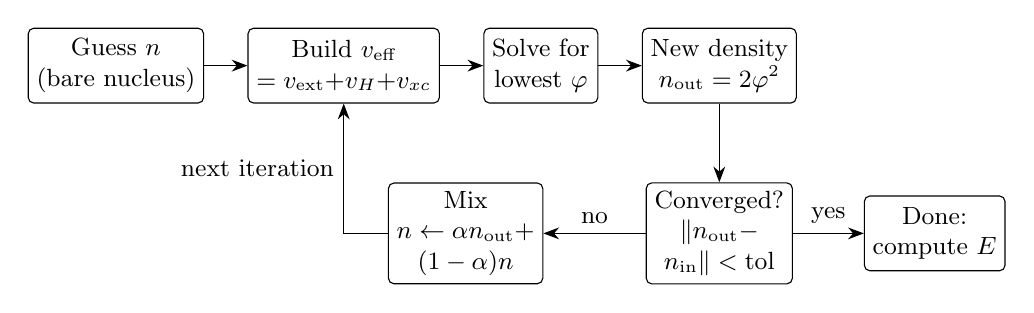
\begin{tikzpicture}[
  box/.style={draw,rounded corners=2pt,align=center,font=\small,minimum height=0.95cm,inner sep=3pt},
  ar/.style={-{Stealth[length=2mm]},thin},
  node distance=0.55cm and 0.55cm]
  \node[box] (guess) {Guess $n$\\(bare nucleus)};
  \node[box,right=of guess] (build) {Build $v_\text{eff}$\\$=v_\text{ext}{+}v_H{+}v_{xc}$};
  \node[box,right=of build] (solve) {Solve for\\lowest $\varphi$};
  \node[box,right=of solve] (dens) {New density\\$n_\text{out}=2\varphi^2$};
  \node[box,below=1.0cm of dens] (conv) {Converged?\\$\|n_\text{out}-$\\$n_\text{in}\|<\text{tol}$};
  \node[box,left=1.3cm of conv] (mix) {Mix\\$n\leftarrow\alpha n_\text{out}+$\\$(1-\alpha)n$};
  \node[box,right=0.9cm of conv] (done) {Done:\\compute $E$};
  \draw[ar] (guess) -- (build);
  \draw[ar] (build) -- (solve);
  \draw[ar] (solve) -- (dens);
  \draw[ar] (dens) -- (conv);
  \draw[ar] (conv) -- node[above,font=\small]{no} (mix);
  \draw[ar] (conv) -- node[above,font=\small]{yes} (done);
  \draw[ar] (mix.west) -| node[pos=0.75,left,font=\small]{next iteration} (build.south);
\end{tikzpicture}
\caption{The self-consistent field loop. In this project $v_{xc}=-\tfrac12v_H$ (exact exchange), which makes
it the Hartree--Fock loop.}
\label{fig:scf}
\end{figure}

\begin{insight}
\textbf{Mixing matters only when the problem is hard.} For helium, plain iteration ($\alpha=1$)
converges in 8 iterations and the fastest mixing was $\alpha=0.9$ (6 iterations, Table~\ref{tab:mix}). For
stretched H$_2$ the same loop fails: at $R=6$, without help, the charge sloshes from one nucleus to the
other and the error is still 2.67 after 300 iterations. Forcing the density to be symmetric under
$x\to-x$ at every step (the exact ground state has this symmetry) makes it converge in 22 iterations at
$\alpha=0.4$. Every H$_2$ result in this report uses the symmetrised loop.
\end{insight}

% =====================================================================
\section{Stretched H\texorpdfstring{$_2$}{2}: static correlation}

Place two nuclei ($Z=1$ each) at $\pm R/2$ and add the nuclear repulsion $w(R)$ to every energy. As
$R\to\infty$ the exact energy tends to two separate hydrogen atoms, $2\times(-0.66986)=-1.33972$\Ha{} on our grid.
Restricted Hartree--Fock keeps one orbital for both electrons. By symmetry it is $\varphi=(\chi_A+\chi_B)/\sqrt2$,
a mix of an orbital on each nucleus, and the product is
\begin{equation}
  \Psi_\text{RHF}=\tfrac12\big[\chi_A(x_1)\chi_A(x_2)+\chi_B(x_1)\chi_B(x_2)+\chi_A(x_1)\chi_B(x_2)+\chi_B(x_1)\chi_A(x_2)\big].
\end{equation}
The last two terms are neutral H\,+\,H. The first two put both electrons on one atom (H$^-$\,+\,H$^+$).
So RHF is 50\% ionic at \emph{every} distance, even when the ionic state costs a lot of energy. This is
\emph{static} (strong) correlation: the true state needs the covalent configuration alone, and one orbital
cannot provide that.

\begin{plainwords}
Two people in two far-apart rooms. The truth is one person per room. Restricted HF insists
that each person is independently ``half in each room'', so half the time both are in the same
room, which is wildly unlikely and costly.
\end{plainwords}

Spin-unrestricted HF fixes the energy by letting each electron localise on one atom, at the cost
of no longer being a proper spin singlet. We did not run it.

% =====================================================================
\section{Results}\label{sec:results}

Every number in this section is printed by \texttt{compare.py}, and every figure is one of its plots. The
label in brackets in each caption (for example ``output 1a'') names the block of its terminal output
that the table comes from. Unless stated otherwise the grid spacing is $h=0.1$ and the box half-width is
$L=10$. ``RHF'' and ``KS with exact exchange'' are the same calculation (Section~\ref{sec:equiv}).

\subsection{Helium and the hydrogen anion}

Table~\ref{tab:atoms} compares total energies. After Richardson extrapolation our solvers reproduce the
problem statement's reference numbers to four decimals (output 3b): one-electron H $=-0.6698$,
He$^+=-1.4834$, exact He $=-2.2383$, RHF $=-2.2242$, $E_c=-0.0140$ and $I=0.7548$\Ha.

\begin{table}[H]
\centering
\begin{tabular}{lrrrr}
\toprule
System & $E_\text{exact}$ & $E_\text{RHF}$ & $\Delta_\text{RHF}=-E_c$ & $\delta_\text{RHF}$ (\%)\\
\midrule
He ($Z=2$), $h=0.1$              & $-2.23855$ & $-2.22450$ & $0.01405$ & $0.63$\\
He ($Z=2$), extrapolated         & $-2.23826$ & $-2.22421$ & $0.01405$ & $0.63$\\
H$^-$ ($Z=1$), $h=0.1$, $L=10$   & $-0.73043$ & $-0.69182$ & $0.03861$ & $5.29$\\
H$^-$ ($Z=1$), $h=0.1$, $L=14$   & $-0.73079$ & $-0.69208$ & $0.03871$ & $5.30$\\
\bottomrule
\end{tabular}
\caption{Total ground-state energies in hartree (outputs 1a, 3b and 4). Extrapolation uses $h=0.1$ and $0.05$.
$\Delta=E_\text{approx}-E_\text{exact}$ and $\delta=100|\Delta|/|E_\text{exact}|$. For Hartree--Fock, $\Delta$ is exactly minus the
correlation energy.}
\label{tab:atoms}
\end{table}

\begin{table}[H]
\centering
\begin{tabular}{lrrrrrrrc}
\toprule
System & $T_s$ & $E_\text{ext}$ & $E_H$ & $E_x$ & $E_{nn}$ & $E$ (terms) & $E$ ($2\varepsilon$ route) & iter.\\
\midrule
H$^-$              & $0.1131$ & $-1.3920$ & $1.1743$ & $-0.5871$ & $0$      & $-0.69182$ & $-0.69182$ & 23\\
He                 & $0.2905$ & $-3.2389$ & $1.4477$ & $-0.7239$ & $0$      & $-2.22450$ & $-2.22450$ & 23\\
H$_2$ ($R=3.5$)    & $0.0965$ & $-2.1652$ & $1.0595$ & $-0.5298$ & $0.2747$ & $-1.26423$ & $-1.26423$ & 19\\
\bottomrule
\end{tabular}
\caption{The Hartree--Fock (= KS exact exchange) energy split into its terms, in hartree (output 1b). The two
routes to $E$ differ by $5\times10^{-8}$, $6\times10^{-8}$ and $1\times10^{-8}$\Ha.}
\label{tab:terms}
\end{table}

\begin{table}[H]
\centering
\begin{tabular}{lrrrr}
\toprule
System & $I=E(\text{one electron})-E(\text{two electrons})$ & $-\varepsilon_\text{HOMO}$ (RHF) & $\Delta$ & $\delta$ (\%)\\
\midrule
He    & $0.7549$ & $0.7503$ & $-0.0046$ & $0.60$\\
H$^-$ & $0.0606$ & $0.0523$ & $-0.0082$ & $13.58$\\
\bottomrule
\end{tabular}
\caption{The HOMO test at $h=0.1$, $L=10$ (output 1c). In exact Kohn--Sham $-\varepsilon_\text{HOMO}=I$; for Hartree--Fock
(Koopmans' theorem) it is only an estimate.}
\label{tab:homo}
\end{table}

\begin{figure}[!htbp]
\centering
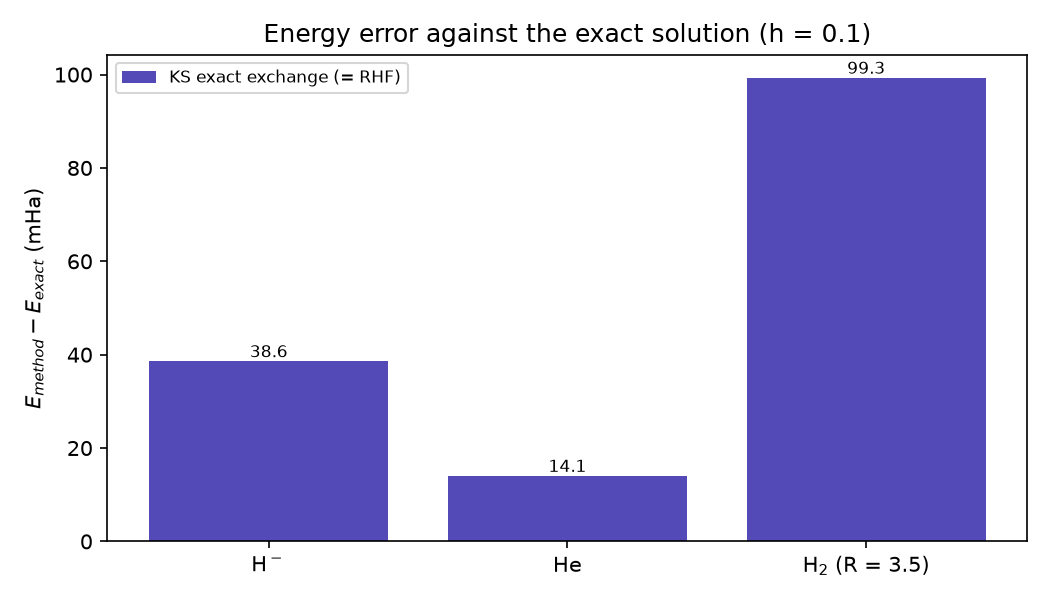
\includegraphics[width=0.72\textwidth]{energy_errors.png}
\caption{Energy error of Hartree--Fock against the exact solution, $E_\text{RHF}-E_\text{exact}=-E_c$, in millihartree.
H$_2$ is at $R=3.5$.}
\label{fig:energy}
\end{figure}

\begin{figure}[!htbp]
\centering
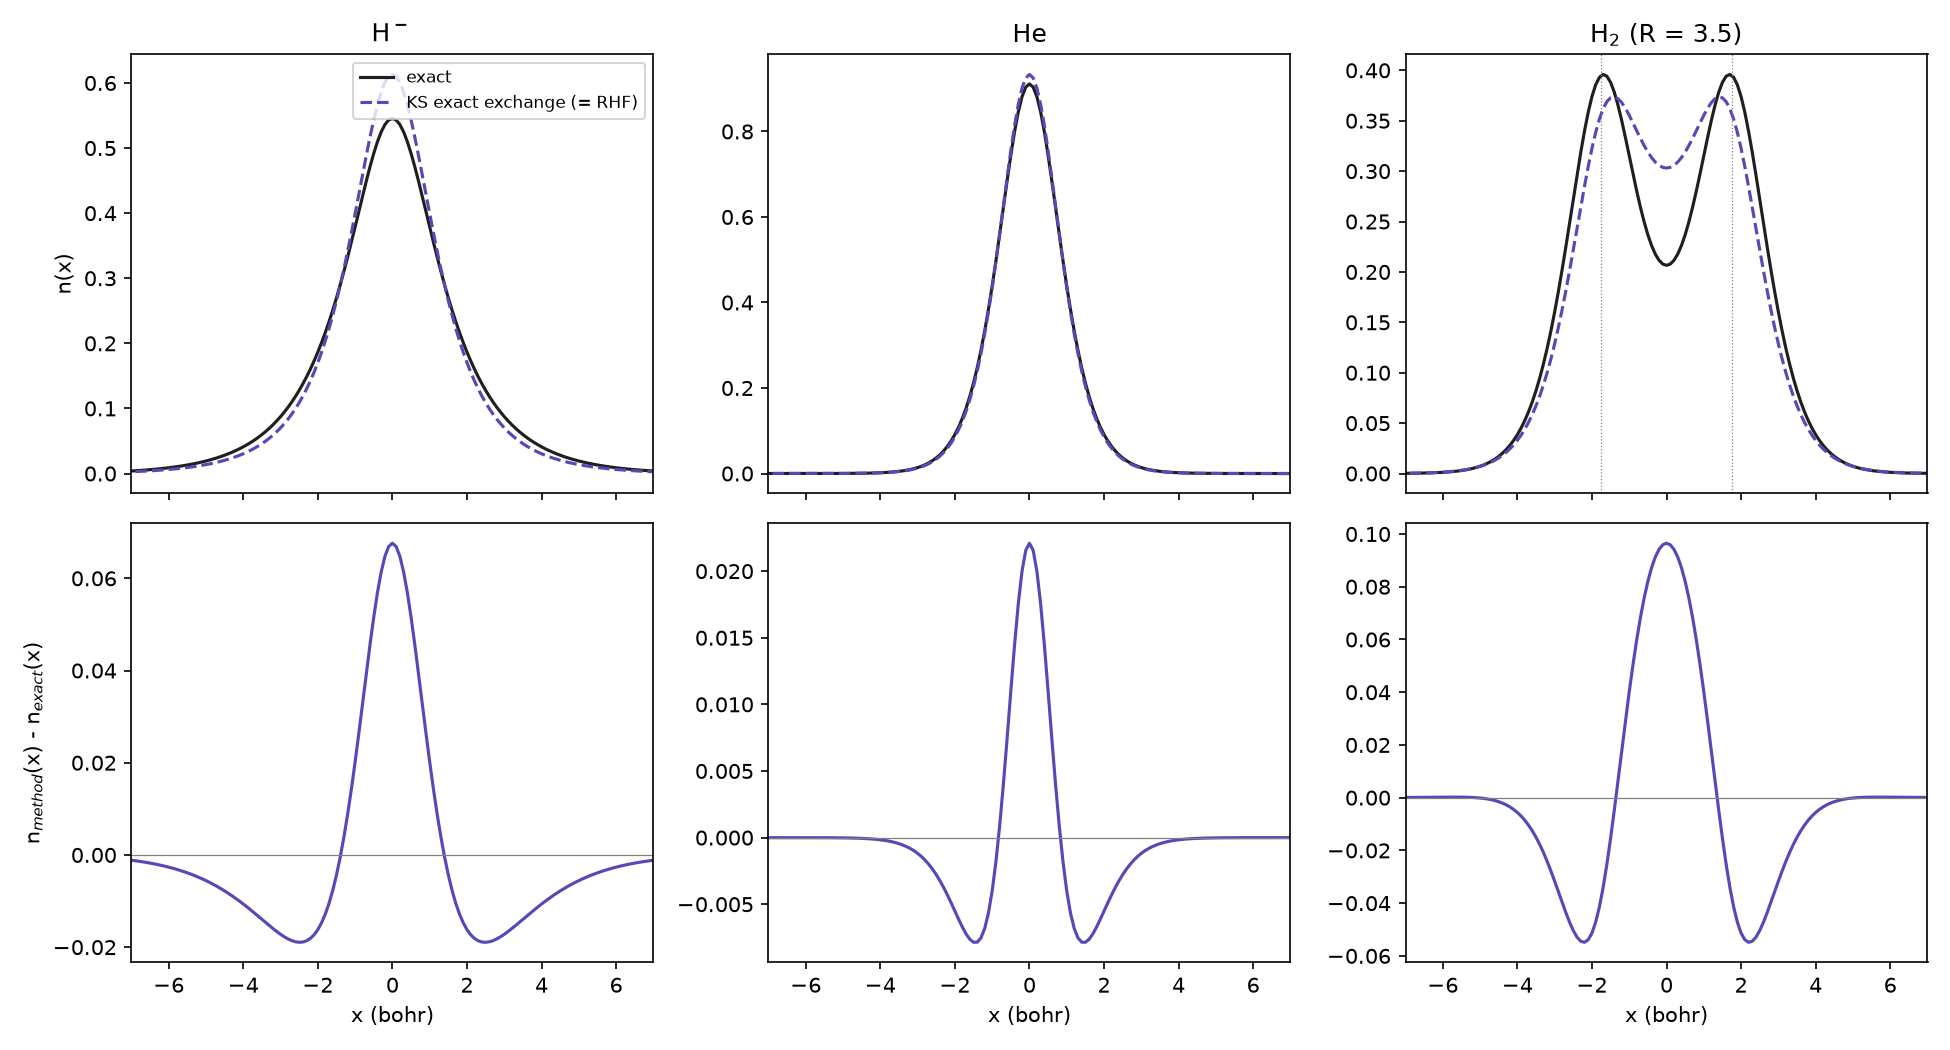
\includegraphics[width=\textwidth]{densities.png}
\caption{Top: ground-state densities, exact (solid) and Hartree--Fock (dashed). Bottom: the difference
$n_\text{RHF}-n_\text{exact}$. Dotted lines mark the nuclei of H$_2$.}
\label{fig:dens}
\end{figure}

\begin{insight}
\textbf{Correlation is small in helium and large in the anion.} The whole correlation energy of He is
only $0.014$\Ha{} (0.63\% of the total), so Hartree--Fock is already very good there. In H$^-$ it is
$0.039$\Ha{}, almost three times larger: the loosely bound electrons have room to avoid each other,
and a product wavefunction cannot describe that avoidance. The densities in Figure~\ref{fig:dens} tell the
same story (output 1d): for He the peaks nearly agree (0.933 against 0.911), while the Hartree--Fock density
of H$^-$ is too compact (peak 0.613 against 0.545).
\end{insight}

\begin{insight}
\textbf{The HOMO test.} The exact $-\varepsilon_\text{HOMO}$ equals the ionisation energy. Hartree--Fock gets helium
to 0.6\% (0.7503 against 0.7549\Ha), because $-\tfrac12v_H$ removes the self-interaction exactly and keeps the
correct $-w(x)$ tail of the potential. For H$^-$ the estimate is off by 14\%: when correlation matters,
Koopmans' theorem is a rough guide.
\end{insight}

\begin{insight}
\textbf{Weakly bound systems are limited by the box.} H$^-$ is bound (exact $E=-0.7304$\Ha{}
below the neutral atom's $-0.6699$\Ha{}, an electron affinity of about 0.06\Ha), but it is so diffuse
that its exact energy still moves by $3.6\times10^{-4}$\Ha{} between $L=10$ and $L=14$ (Table~\ref{tab:box}).
Helium is converged to $10^{-6}$\Ha{} by $L=8$.
\end{insight}

\subsection{Grid and box convergence}

\begin{table}[H]
\centering
\begin{tabular}{lrrrr}
\toprule
$h$ (bohr) & $E_\text{exact}$(He) & ratio & $E_\text{RHF}$(He) & ratio\\
\midrule
0.4          & $-2.243017$ & --   & $-2.228938$ & --\\
0.2          & $-2.239430$ & --   & $-2.225374$ & --\\
0.1          & $-2.238550$ & 4.07 & $-2.224500$ & 4.08\\
0.05         & $-2.238331$ & 4.02 & $-2.224282$ & 4.02\\
extrapolated & $-2.238258$ & --   & $-2.224209$ & --\\
\bottomrule
\end{tabular}
\caption{Grid-spacing convergence of the helium energy at $L=10$, in hartree (output 3a). The ratio of successive
differences is 4 when the error is $\propto h^2$. Extrapolation uses $h=0.1$ and $0.05$.}
\label{tab:grid}
\end{table}

The observed order of convergence, from \texttt{convergence\_order}, is $p=2.03$ and $2.01$ for both solvers, as
expected for a three-point second derivative.

\begin{table}[H]
\centering
\begin{tabular}{lrrrr}
\toprule
$L$ (bohr) & $E_\text{exact}$(He) & $E_\text{exact}$(H$^-$) & $E_\text{RHF}$(H$^-$) & $-\varepsilon_\text{HOMO}$(H$^-$)\\
\midrule
6  & $-2.238506$ & $-0.723313$ & $-0.686460$ & $0.0394$\\
8  & $-2.238549$ & $-0.729191$ & $-0.690923$ & $0.0492$\\
10 & $-2.238550$ & $-0.730432$ & $-0.691823$ & $0.0523$\\
12 & $-2.238550$ & $-0.730721$ & $-0.692031$ & $0.0534$\\
14 & $-2.238550$ & $-0.730790$ & $-0.692082$ & $0.0538$\\
\bottomrule
\end{tabular}
\caption{Box-size convergence at $h=0.1$, energies in hartree (output 4). Helium is converged by $L=8$; H$^-$ is still
drifting at $L=14$.}
\label{tab:box}
\end{table}

\subsection{SCF mixing}

\begin{table}[H]
\centering
\begin{tabular}{lrrrrrrrrrr}
\toprule
$\alpha$ & 0.1 & 0.2 & 0.3 & 0.4 & 0.5 & 0.6 & 0.7 & 0.8 & 0.9 & 1.0\\
\midrule
He              & 110 & 52 & 33 & 23 & 17 & 13 & 10 & 7 & 6 & 8\\
H$_2$ ($R=3.5$) & 91  & 43 & 27 & 19 & 14 & 11 & 8  & 8 & 12 & 17\\
\bottomrule
\end{tabular}
\caption{SCF iterations to reach $\|n_\text{out}-n_\text{in}\|<10^{-6}$ against the mixing parameter $\alpha$ (output 5a).}
\label{tab:mix}
\end{table}

Helium converges for every $\alpha$, fastest just below 1. For H$_2$ at $R=3.5$ the optimum is
$\alpha\approx0.7$--$0.8$, and plain iteration ($\alpha=1$) is already twice as slow: the extra overshoot between
the two nuclei is the first sign of the sloshing that stops stretched H$_2$ converging at all
unless the density is symmetrised (output 5b).

\subsection{Stretched H\texorpdfstring{$_2$}{2}}

\begin{table}[H]
\centering
\begin{tabular}{rrrrrrr}
\toprule
$R$ & $E_\text{exact}$ & $E_\text{RHF}$ & $\Delta_\text{RHF}=-E_c$ & $\delta_\text{RHF}$ (\%) & $E_{nn}=w(R)$ & exact electronic\\
\midrule
1.0  & $-1.41320$ & $-1.39452$ & $0.01868$ & 1.32  & 0.70711 & $-2.12030$\\
1.5  & $-1.45172$ & $-1.42639$ & $0.02533$ & 1.74  & 0.55470 & $-2.00642$\\
2.0  & $-1.44200$ & $-1.40591$ & $0.03609$ & 2.50  & 0.44721 & $-1.88921$\\
2.5  & $-1.41356$ & $-1.36158$ & $0.05198$ & 3.68  & 0.37139 & $-1.78495$\\
3.0  & $-1.38483$ & $-1.31146$ & $0.07338$ & 5.30  & 0.31623 & $-1.70106$\\
4.0  & $-1.35067$ & $-1.22322$ & $0.12745$ & 9.44  & 0.24254 & $-1.59321$\\
5.0  & $-1.34091$ & $-1.16115$ & $0.17976$ & 13.41 & 0.19612 & $-1.53703$\\
6.0  & $-1.33930$ & $-1.12054$ & $0.21876$ & 16.33 & 0.16440 & $-1.50370$\\
8.0  & $-1.33946$ & $-1.07697$ & $0.26249$ & 19.60 & 0.12403 & $-1.46350$\\
10.0 & $-1.33963$ & $-1.05706$ & $0.28257$ & 21.09 & 0.09950 & $-1.43913$\\
\bottomrule
\end{tabular}
\caption{Stretched 1D H$_2$ at $h=0.1$, with box half-width $L=\max(10,\,R/2+9)$, energies in hartree (output 2a).
$E_\text{exact}$ and $E_\text{RHF}$ are total energies (electronic energy plus $E_{nn}$); the last column is the exact
electronic energy alone. Mean absolute error of RHF over the 10 distances: 0.1276\Ha.}
\label{tab:h2}
\end{table}

\begin{figure}[!htbp]
\centering
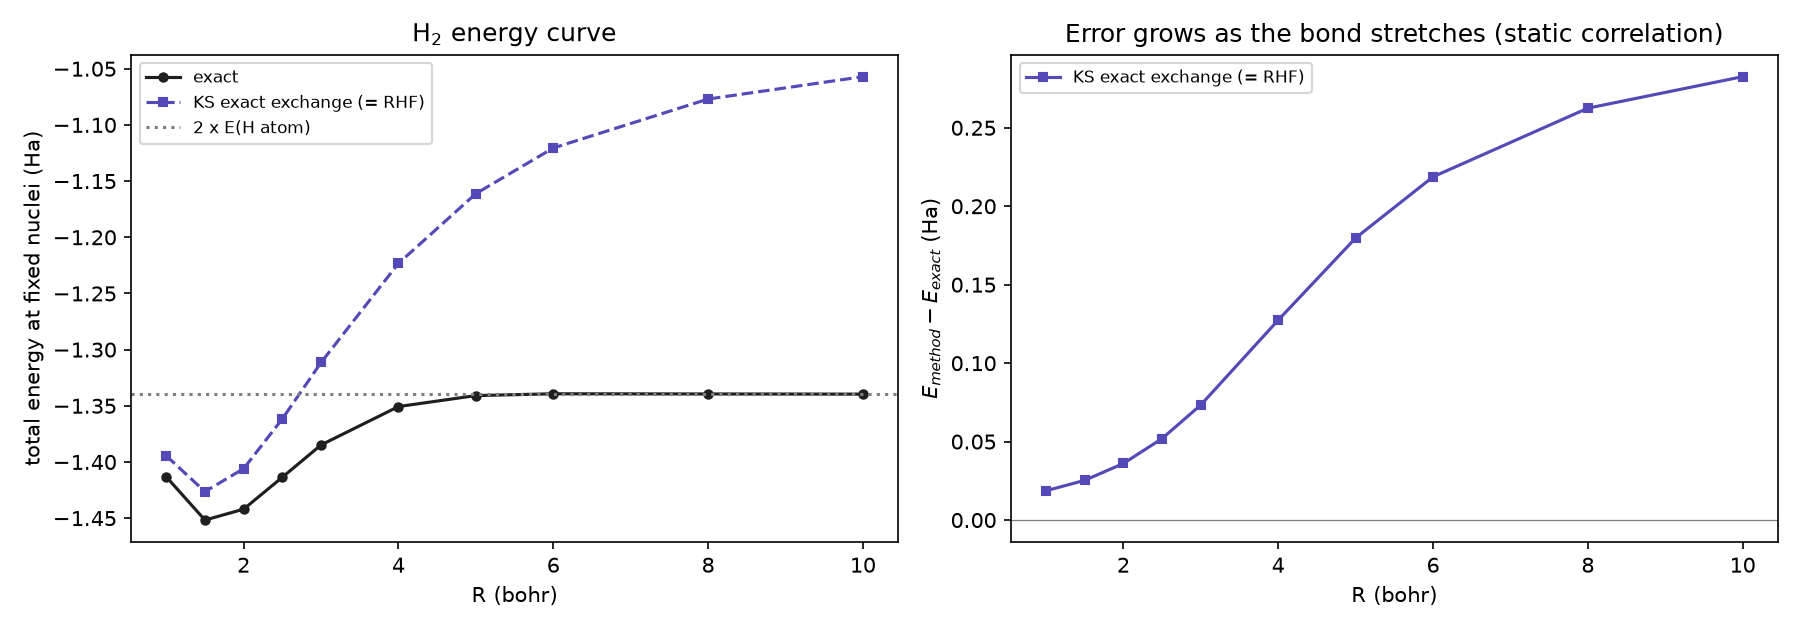
\includegraphics[width=\textwidth]{H2_energy_curve.png}
\caption{Left: the H$_2$ total-energy curve. The exact curve has its minimum near $R\approx1.5$--$2$ and dissociates to
two H atoms ($-1.33972$\Ha, grey line); RHF stays far too high. Right: the RHF error, which equals $|E_c|$
and grows to 0.28\Ha.}
\label{fig:h2}
\end{figure}

\begin{insight}
\textbf{Stretching the bond is a qualitative failure, not a small error.} The RHF error rises
from 0.019\Ha{} at $R=1$ to 0.283\Ha{} at $R=10$ and is still rising. The exact wavefunction shows why
(output 2b): at $R=3.5$ the probability that both electrons sit on the same side of the molecule is 0.145
in the exact $\Psi$ and 0.485 in the RHF product, close to the 50\% that Section~6 predicts. The lesson:
say ``approximate methods fail'', not ``the theory fails''.
\end{insight}

\subsection{Agreement with the problem statement's reference table}

The exact column of our stretched-H$_2$ table matches the problem statement's reference at
$R=1,2,4,6,10$ to within about $2\times10^{-4}$\Ha, the size expected from its coarser grid ($h=0.15$).
The RHF column matches at $R=1,2$ but not beyond (Table~\ref{tab:ref}).

\begin{table}[H]
\centering
\begin{tabular}{rrr}
\toprule
$R$ & RHF (reference table) & RHF (this work)\\
\midrule
4  & $-1.1904$ & $-1.2232$\\
6  & $-1.0693$ & $-1.1205$\\
10 & $-1.0224$ & $-1.0571$\\
\bottomrule
\end{tabular}
\caption{Where the stretched-H$_2$ Hartree--Fock numbers differ from the table that came with the problem
statement. All values in Ha; ``this work'' is output 2a.}
\label{tab:ref}
\end{table}

Restricted Hartree--Fock is variational, so a lower converged energy means a better restricted state.
We reproduced the likely cause ourselves: without the symmetrised density the loop does not converge
for stretched H$_2$, because the charge sloshes between the nuclei. The reference RHF values for
$R\ge4$ were most likely taken from such an unconverged loop. We cannot check how that table was
produced, so this remains our best explanation rather than a proof.

\begin{insight}
\textbf{Verify, then trust.} Checking every energy by two routes, and checking the variational ordering
$E_\text{RHF}\ge E_\text{exact}$, caught a disagreement with a reference table. The same discipline found the bugs
of our first notebook: two different softening lengths in one Hamiltonian (0.2 for the electron
repulsion of H$_2$, 0.001 in one H$^-$ run), a grid spacing hard-coded separately from the grid,
the Kohn--Sham loop borrowing the exact solver's grid, and a missing nuclear repulsion. Use one softening
parameter for every interaction and derive $h$ from the grid.
\end{insight}

% =====================================================================
\section{Error analysis}

\subsection{Definitions}

Let $E_\text{exact}$ be the exact value on the same grid and $E_\text{approx}$ the value from a method. The signed
error and the relative error are
\begin{equation}
  \Delta=E_\text{approx}-E_\text{exact},\qquad \delta=\frac{|\Delta|}{|E_\text{exact}|}\times100\%.
\end{equation}
The sign matters. Hartree--Fock is variational, so $\Delta_\text{RHF}\ge0$ must hold for every system on the
same grid. All our values satisfy this, which is a useful sanity check.

\textbf{Error of the correlation energy.} By definition $E_c=E_\text{exact}-E_\text{HF}$, so
\begin{equation}
  \Delta_\text{RHF}=E_\text{HF}-E_\text{exact}=-E_c=|E_c|.
\end{equation}
The RHF error \emph{is} the correlation energy.

\textbf{Error of an orbital energy.} Because $-\varepsilon_\text{HOMO}$ should equal $I=E(\text{ion})-E(\text{atom})$, we use
$\Delta=(-\varepsilon_\text{HOMO})-I$.

\textbf{Mean absolute error over several points.} For $n$ bond lengths,
\begin{equation}
  \text{MAE}=\frac1n\sum_{i=1}^n|\Delta_i|.
\end{equation}
Over the 10 distances of Table~\ref{tab:h2}, $\text{MAE}_\text{RHF}=0.1276$\Ha.

\subsection{Numerical (discretisation) uncertainty}

Richardson extrapolation provides its own error estimate (output 3a). The un-extrapolated error of $E(h)$ is
about $|E(h)-E(2h)|/3$, which is $0.29$\,mHa for helium at $h=0.1$. A second estimate of the remaining error
is the difference between two extrapolations, from $(0.2,0.1)$ and from $(0.1,0.05)$. For helium these are
$-2.238256$ and $-2.238258$\Ha, so the extrapolated energy is good to about $10^{-6}$\Ha. The H$_2$ energies
are not extrapolated; at $h=0.1$ their grid error should be a few $10^{-4}$\Ha, similar to helium.

\textbf{Propagation.} If $E_\text{exact}$ and $E_\text{HF}$ each carry an independent uncertainty $\sigma$, then
\begin{equation}
  \sigma_{E_c}=\sqrt{\sigma_\text{exact}^2+\sigma_\text{HF}^2}\ \ (\text{independent}),\qquad
  \sigma_{E_c}\le\sigma_\text{exact}+\sigma_\text{HF}\ \ (\text{worst case}).
\end{equation}
Because both solvers use the same grid, much of the $h^2$ error cancels in the difference, so $E_c$ is
more accurate than either energy alone: it is $-0.01405$\Ha{} both at $h=0.1$ and after extrapolation (output 3b).
All quoted errors $\Delta$ are far larger than these numerical uncertainties, except for the box-limited H$^-$.

\subsection{Summary of results and errors}

\begin{table}[H]
\centering
\begin{tabular}{llrrrr}
\toprule
Quantity & Method & Exact & Value & $\Delta$ & $\delta$ (\%)\\
\midrule
He total energy (extrapolated)        & RHF & $-2.2383$ & $-2.2242$ & $0.0140$  & 0.63\\
He $-\varepsilon_\text{HOMO}$ vs $I$             & RHF & $0.7549$  & $0.7503$  & $-0.0046$ & 0.60\\
H$^-$ total energy ($L=10$)            & RHF & $-0.7304$ & $-0.6918$ & $0.0386$  & 5.29\\
H$^-$ $-\varepsilon_\text{HOMO}$ vs $I$ ($L=10$) & RHF & $0.0606$  & $0.0523$  & $-0.0082$ & 13.58\\
H$_2$ total energy, $R=2$              & RHF & $-1.4420$ & $-1.4059$ & $0.0361$  & 2.50\\
H$_2$ total energy, $R=3.5$            & RHF & $-1.3636$ & $-1.2642$ & $0.0993$  & 7.28\\
H$_2$ total energy, $R=10$             & RHF & $-1.3396$ & $-1.0571$ & $0.2826$  & 21.09\\
\bottomrule
\end{tabular}
\caption{Summary of the comparison with the exact solution (all values in Ha, outputs 1a, 1c, 2a and 3b).
$\Delta=\text{value}-\text{exact}$, $\delta=100|\Delta|/|\text{exact}|$.}
\label{tab:summary}
\end{table}

\begin{insight}
\textbf{Reading the table.} Hartree--Fock is excellent for the tightly bound atom (0.63\% total-energy
error, 0.6\% on $I$) because it removes self-interaction exactly and only misses correlation. It is
noticeably worse for the diffuse anion (5.3\%), and it is not reliable once the bond is stretched, where
the error reaches 21\% of the total energy. Every one of these errors is pure correlation, measured
exactly, which is what makes this toy model a useful benchmark for any functional that comes next.
\end{insight}

% =====================================================================
\section{Future direction}\label{sec:future}

None of this section was implemented; it is the plan for the phases we did not reach.

\textbf{LDA exchange (Phase 4).} The local density approximation treats every small slice of the system
as a piece of uniform electron gas at the local density~\cite{capelle,harrison}. A uniform 1D gas has $k_F=\pi n/2$ and density matrix
$\gamma(x)=(k_F/\pi)\sin(k_Fx)/(k_Fx)$ per spin. Putting $\gamma^2$ into the exchange integral and substituting $t=k_Fx$ gives
\begin{equation}
  n\,e_x(n)=-\int_{-\infty}^{\infty}w(x)\,\gamma(x)^2\dd x=-\frac{n^2}{2}J\!\left(\frac{\pi n}{2}\right),\qquad
  J(k)=\int_0^\infty\frac{\sin^2t}{t^2\sqrt{t^2+k^2}}\dd t,
\end{equation}
with $E_x^\text{LDA}=\int n\,e_x(n)\dd x$ and $v_x(n)=\dd[n\,e_x(n)]/\dd n$. At high density $J\approx\pi/(2k_F)$, so
$e_x\to-\tfrac12$, which is the check the problem statement asks for. $J$ has no closed form, so it would be tabulated
once and splined in $\ln n$. In our SCF loop only one line would change: $v_\text{eff}=v_\text{ext}+v_H+v_x(n)$ instead of
$v_\text{ext}+\tfrac12v_H$. The problem statement's reference calculation gives $-2.158$\Ha{} for 1D helium with LDA
exchange, and an exchange energy of $-0.654$\Ha{} against the exact-exchange $-0.724$\Ha. If that holds, LDA
misses about 10\% of the exchange, several times the whole correlation energy we measured ($-0.014$\Ha).

\begin{plainwords}
LDA is like valuing hilly farmland by treating every small patch as flat land at that patch's
altitude. It is fine where the land changes slowly and wrong near cliffs. Atoms are full of
cliffs, because the density drops quickly.
\end{plainwords}

\textbf{Exact $v_{xc}$ by inversion (Phase 6).} For two electrons the Kohn--Sham orbital is exactly $\varphi=\sqrt{n/2}$,
so our exact density gives the exact potential with no iteration:
$v_{xc}=\varepsilon+\varphi''/(2\varphi)-v_\text{ext}-v_H$, with $\varepsilon=-I$. Its tail should follow $-w(x)$, while LDA's dies
exponentially, and for stretched H$_2$ it should grow a peak at the bond midpoint that no local functional
can reproduce.

\textbf{Also left to do.} LDA correlation (Phase 5); the $Z$ scan (our one-nucleus solvers already take \texttt{Z});
the softening scan; unrestricted Hartree--Fock for stretched H$_2$; and timing the solvers against grid size to
measure the scaling of Section~2.

% =====================================================================
\section{Conclusions}

\textbf{What we achieved.}
\begin{enumerate}
  \item The exact two-electron solver works for H$^-$, He and H$_2$, reproduces every reference value of
        the problem statement for the atoms, and is a trustworthy yardstick (about $10^{-6}$\Ha{} for
        extrapolated He).
  \item Hartree--Fock (= Kohn--Sham with exact exchange) is implemented for the same systems. Two
        independent energy routes agree, and the variational ordering holds everywhere.
  \item The exact correlation energy follows directly: $-0.014$\Ha{} for He, $-0.039$\Ha{} for H$^-$, and up to
        $-0.28$\Ha{} for stretched H$_2$, where restricted Hartree--Fock fails qualitatively because of static
        correlation.
  \item The numerical side is under control and reproducible from \texttt{compare.py}: $h^2$ convergence with
        Richardson extrapolation, box size, SCF mixing, and the charge-sloshing failure of stretched H$_2$ (and its fix).
\end{enumerate}

\textbf{What we could not do.} We did not implement LDA (Phase 4), LDA correlation (Phase 5) or the exact
exchange--correlation potential (Phase 6). So the project's central question, \emph{where approximate DFT fails},
is answered only for the special functional ``exact exchange, no correlation''. Section~\ref{sec:future} describes
how the remaining phases would be done.

% =====================================================================
{\small
\begin{thebibliography}{9}
\addcontentsline{toc}{section}{References}

\bibitem{kohn}
W.~Kohn, \emph{Electronic structure of matter --- wave functions and density functionals},
Nobel Lecture, 28 January 1999.
\url{https://www.nobelprize.org/uploads/2018/06/kohn-lecture.pdf}

\bibitem{capelle}
K.~Capelle, \emph{A bird's-eye view of density-functional theory}, arXiv:cond-mat/0211443.
\url{https://arxiv.org/pdf/cond-mat/0211443}

\bibitem{harrison}
N.~M.~Harrison, \emph{An introduction to density functional theory}, lecture notes, Imperial College
London and CLRC Daresbury Laboratory.
\url{https://www.imperial.ac.uk/media/imperial-college/research-centres-and-groups/computational-materials-science/teaching/DFT_NATO.pdf}

\end{thebibliography}
}

\end{document}
